\section{Scattering}
\subsection{Classical scattering}
In scattering problems, we assume a spatially and temporally uniform distribution of 
incoming beams along the incident axis. We also assume cylindrical 
symmetry parameterized by $(z, b, \phi)$ denoting height, radius, and 
azimuthal angle, respectively. Below are the quantities involved 
in the problem. 
\begin{itemize}
    \item Impact prameter $b$, scattering angle $\theta$.
    \item Particles incident within an infinitesimal patch 
    of cross-sectional area $d\sigma = b\, db\, d\varphi$ scatters into a 
    solid angle (normalized area form) $d\Omega = \sin\theta \, d\theta\, d\varphi$. 
    \item Differential cross-section 
    $d_\Omega \sigma = \df b {\sin\theta}\left|d_\theta b \right|$. 
    Usually, the greater $\theta$ (more pronounced scattering), the smaller $b$, thus 
    the absolute sign. $d_\Omega \sigma$ is usually a 
    quantity parameterized by $\theta$. It asks: at angle $\theta$ 
    from the scattering center, how much unit solid angle accounts 
    for unit area increase in incident beams? 
    \item The total cross-section $\sigma = \int d_\Omega \sigma\, d\Omega$. It is 
    the total cross-sectional area which will encounter scattering. For classical hard-sphere 
    scattering, this is $\pi R^2$. 
    \item The luminosity $\mathcal L$ is the experimentally controllable 
    parameter denoting the number of incident particles 
    per unit cross-sectional area, per unit time. We have 
    $dN = \mathcal L\, d\sigma$, so 
    $d_\Omega\sigma = \df 1 {\mathcal L} d_\Omega N$
\end{itemize}
\begin{figure}[h!] % The [h!] tries to place the figure "here" as closely as possible
    \centering
    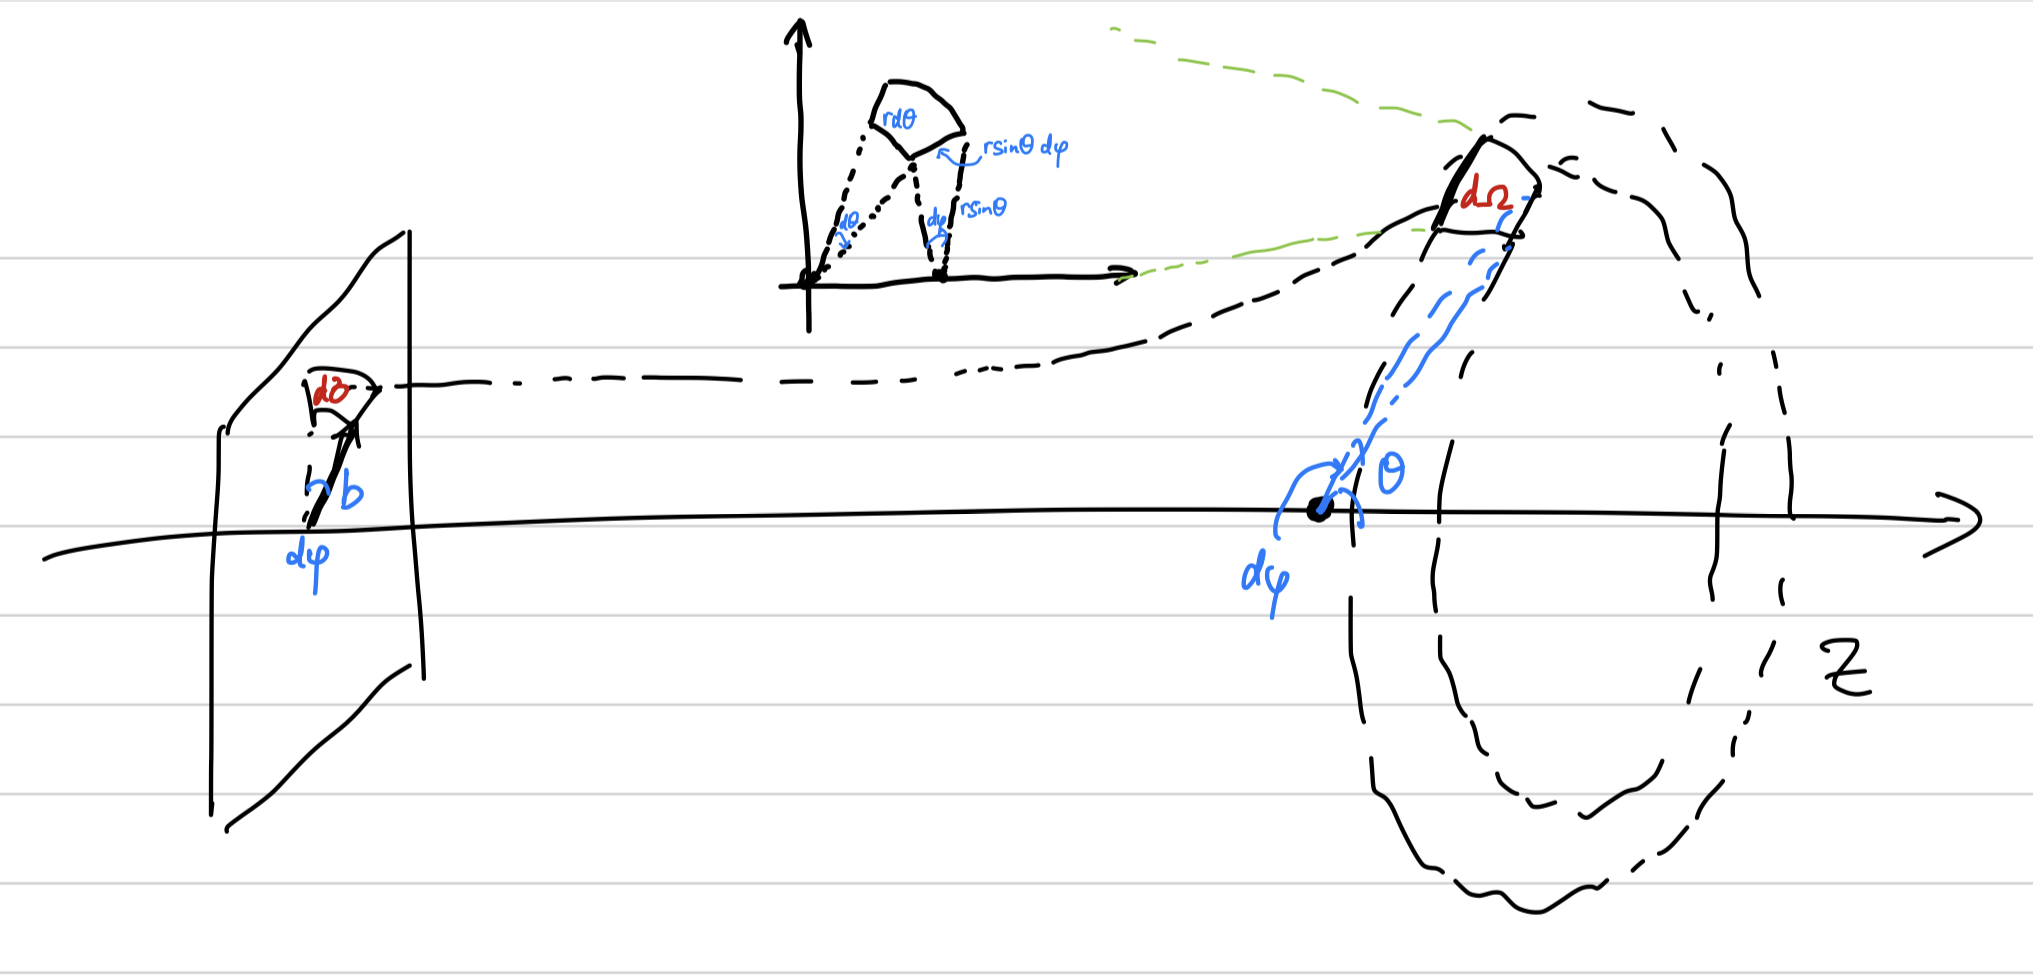
\includegraphics[width=1\linewidth]{src/scattering.jpeg}
    % \caption}
    \label{fig:scattering}
\end{figure}



\subsection{Quantum scattering theory}
Assuming that the scattering potential is localized and spherically symmetric, 
it admits separable solutions 
\[ 
    \psi(r, \theta, \phi) = \sum_{l, m} \df{u_{m, l}(r)}{r} Y^m_l(\theta, \phi)
\] 
Here $u$ satisfies one-dimensional radial equation with effective potential 
\leqalign{eqn:radial se}{
    -\df{\hb^2}{2m} \pd r^2 u + \left[V(r) + \df{\hb^2}{2m} \df{L^2}{r^2}\right]u = Eu 
}
For asymptotically large $kr\gg 1$, the effective potential converges to the radial potential, 
which gives the general solution 
\[ 
    \psi(r, \theta, \phi) = \df{Y^m_l(\theta, \phi)}r\left(Ce^{ikr} + De^{-ikr}\right)
\] 
The outgoing scattering condition eliminates $D$. Our potential starts out 
with both polar and azimuthal symmetry. 
Incidence direction chooses a preferred $z$-axis and 
introduces $\theta$ dependence by breaking spherical symmetry
However, the azimuthally symmetric incidence condition 
leaves our state $\phi$-invariant. 
The only $\phi$-invariant spherical harmonics are those with $m=0$, so 
we look for steady state solutions for $r\gg 1$ of the following form: 
\begin{mdframed}
\leqalign{eqn:radiation state}{
    \psi(r, \theta) = 
    A\left[e^{ikz}+\left(\sum_{l=0}^\infty c_l Y^0_l(\theta)\right)\df{e^{ikr}}{r}\right]
    ,\quad k = \df{2mE}{\hb}
}
\end{mdframed}
The spherically normalized amplitudes in parantheses are collected into the 
\textit{scattering amplitude} $f(\theta)$. 
The probability flux of a uniform 
beam through cross-sectional area $d\sigma$ is 
\[ 
    dP = |\psi_{\mrm{incident}}|^2\, d\sigma = |A|^2 \, d\sigma 
\] 
This is equal to the probability that it scatters into the 
corresponding solid angle $d\Omega$: 
\[ 
    dP = |\psi_{\mrm{scattered}}|^2\, d\Omega = \df{|Af|^2}{r^2} (r^2\, d\Omega)
    = |Af|^2\, d\Omega 
\] 
The differential cross-section is correspondingly 
\[ 
    d_\Omega \sigma = |f(\theta)|^2
\] 
The subsequent subsections introduce two methods to compute the 
scattering amplitudes. 


\subsection{Partial wave analysis}
Partial wave analysis allows us to calculate the scattering amplitudes 
for localized $V(r)$ which \textit{decays faster than $r^2$} 
(this includes finite-range potentials). 

Consider equation~\ref{eqn:radial se} again. 
When $V(r)$ decays faster than $r^{-2}$, our space 
can be split into three regions of interest 
(note that Coulomb potential is not well-localized in this sense). 
\begin{itemize}
    \item scattering region: $V\neq 0$ and $kr\gg 1$. Here a full consideration 
    is needed. 
    \item intermediate region: $V(r)\approx 0$ but the centrifugal term 
    $\df{\hb^2}{2m} \df{L^2}{r^2}$ is still nonneglegible. The particle is radially ``free". 
    \item radiation zone:  $kr\gg 1$, so both $V(r)$ and the centrifugal terms are neglegible. 
    The state in this regime is given by equation~\ref{eqn:radiation state}.
\end{itemize}
We consider the intermediate region, equation~\ref{eqn:radial se} becomes 
\leqalign{eqn:intermediate region se}{
    u(r) = Arj_l(kr) + Brn_l(kr)
}
Here $n_l, j_l$ are the spherical Bessel functions which somewhat represents 
sines and cosines. It is more helpful to change basis to linear combinations 
of the Bessels representing the analogue of complex exponentials, or the 
\textit{spherical Hankel functions} which are asymptotically $e^{\pm ikx}/r$
\[ 
    h_l^{(1)}(x) \equiv j_l(x) + in_l(x), \quad h_l^{(2)}(x) = j_l(x) - in_l(x)
\] 
Outgoing solutions are represented by Hankel functions of the first kind, 
so the intermediate region's state is of the form 
\[ 
    \psi(r, \theta) = A\left[e^{ikz} + \sum c_{m, l} Y^m_l(r, \theta)R_l(r)\right] = 
    A\left[e^{ikz} + \sum_{l=0}^\infty c_l h_l^{(1)}(kr) Y_l^0(\theta)\right]
\] 
Redefine expansion coefficients with the \textit{$l$-th partial wave 
amplitude} $c_l = i^{l+1}k\sqrt{4\pi(2l+1)}a_l$; this parameterization turns 
out to be useful later. Substituting $Y_l^0(\theta)$ yields 
\[ 
    \psi(r, \theta) = A\left[e^{ikz} + 
    k\sum_{l=0}^\infty i^{l+1}(2l+1)a_lh^{(1)}_l(kr) P_l(\cos\theta)\right]
\] 
To use consistent spherical coordinates, we need to use Rayleigh's formula 
\leqalign{eqn:Rayleigh's formula}{
    e^{ikz} = \sum_{l=0}^\infty i^l(2l+1)j_l(kr)P_l(\cos\theta)
}
The intermediate region's state is then of the form 
\begin{mdframed}
    \leqalign{eqn:intermediate region se}{
        \psi(r, \theta) = A
        \sum_{l=0}^\infty i^{l}(2l+1)\left[j_l(kr) 
        + i k a_lh^{(1)}_l(kr)\right] P_l(\cos\theta)
    }
    \end{mdframed}
The $l$-th partial wave amplitudes $a_l$ are so defined because for 
large $r$, the Hankel functions approach $(-i)^{l+1}e^{ikr}/kr$, so 
equation~\ref{eqn:intermediate region se} approaches 
equation~\ref{eqn:radiation state} with 
\[ 
    f(\theta) = \sum_{l=0}^\infty c_l Y^0_l(\theta)
    = \sum_{l=0}^\infty (2l+1)a_lP_l(\cos\theta)
\] 
The differential cross-section can be computed from the partial wave amplitudes by 
\leqalign{eqn:quantum differential cross section}{
    d_\Omega \sigma(\theta) = |f(\theta)|^2 = 
    \sum_{l, l'}(2l+1)(2l'+1)a_l^*a_{l'}P_l(\cos\theta)P_{l'}(\cos\theta)
}
Integrate over the solid angle to obtain the total cross section 
\leqalign{eqn:quantum total cross section}{
    d_\Omega \sigma(\theta) = |f(\theta)|^2 = 
    4\pi \sum_{l=0}^\infty (2l+1)|a_l|^2
}
When the centrifugal term dominates over the radial potential, 
the partial wave components are dominated by components with low angular 
momentum. 

For an algorithmic prescription of partial wave analysis: 
\begin{itemize}
    \item Choose a potential cutoff $R$ beyond which to use 
    equation~\ref{eqn:quantum differential cross section}. 
    Solve for the eigenstates of the potential for $r\leq R$. 
    \item Use matching boundary conditions to evaluate $a_l$. 
    \item Use the partial wave amplitudes to calculate quantities of interest. 
    If possible, for infinite-range but quickly-decaying potentials take $R\to \infty$. 
\end{itemize}


% \subsection{Phase shifts}
% The whole story simplifies considerably when the potential is spherically 
% symmetric. This implies that angular momentum is conserved and each partial wave 
% below is independently scattered with no change in amplitude, only in phase. 
% We consider this rigorously 
% \[ 
%     \psi^{(l)} = A i^l(2l+1)j_l(kr)P_l(\cos\theta), \quad V(r) = 0
% \] 
% For large $r$, this takes the asymptotic form 
% \[ 
%     \psi^{(l)} \approx A\df{(2l+1)}{2ikr}\left[e^{ikr} - (-1)^l e^{-ikr}\right]P_l(\cos\theta)
% \] 

\subsection{Integral form of the eigenvalue equation}
The three-dimensional eigenvalue equation for the Hamiltonian may be rewritten as 
\leqalign{eqn:3d se}{
    (\nabla^2 + k^2)\psi(\mbf r) = \df{2m}{\hb^2}V(\mbf r)\psi(\mbf r), 
    \quad k = \df{\sqrt{2mE}}{\hb}
}
This has the superficial apearance of a Helmholtz equation
\[ 
    \left(\nabla^2 + k^2\right)\psi = Q, \quad Q(\mbf r) = \df{2m}{\hb^2}V(\mbf r)\psi(\mbf r)
\] 
However, the important difference is that the inhomogeneous term $Q$ 
now also depends on $\psi$. Recall that given a 
Green function $G(\mbf r)$ which solves the Helmholtz equation with a 
delta function ``source'', integrating it gives the solution 
to the Helmholtz equation. 
\leqalign{eqn:green condition}{
    (\nabla^2 + k^2)G(\mbf r) = \delta^3(\mbf r)
}
While a Green function will not allow us to write the closed form 
to the eigenvalue equation, it yields an equivalent equation 
(note that $\psi$ also appears on the right hand side). 
\[ 
    \psi(\mbf r) = \int d^3\mbf r' \, 
    Q(\mbf r') G(\mbf r - \mbf r')
\] 
To see that this equation is equivalent to equation~\ref{eqn:3d se}, 
apply $(\nabla^2+k^2)$ to both sides. 
\[ 
    (\nabla^2 + k^2)\psi(\mbf r) = 
    \int d^3\mbf r'\left(\nabla^2 + k^2\right)G(\mbf{r - r'}) Q(\mbf r') 
    = \int \delta(\mbf{r-r'})Q(\mbf r')\, d^3\mbf r' = Q(\mbf r)
\] 
One Green function which satisfies equation~\ref{eqn:green condition} is 
\[ 
    G(x) = -\df{e^{ikr}}{4\pi r}
\] 
The free part of the eigenvalue equation solution is the kernel 
of $\nabla^2+k^2$ corresponding to the free-particle solutions. 
This allows us to write the general integral form of equation~\ref{eqn:3d se}. 
\begin{mdframed}
\leqalign{eqn:integral se}{
    \psi(\mbf r) = \psi_0(\mbf r) - 
    \df{m}{2\pi \hb^2}\int \df{e^{ik|\mbf r - \mbf r'|}}{|\mbf r - \mbf r'|}
    V(\mbf r')\psi(\mbf r')d^3\mbf r', \quad  (\nabla^2+k^2)\psi_0(\mbf r) = 0
}\end{mdframed}


\subsection{Born Approximation}
Suppose $V$ is localized about $\mbf r'=0$ 
and we wish to calculate $\psi(\mbf r)$ for points far away from the scattering center. 
The contributing terms all satisfy $|\mbf r'|\ll |\mbf r|$, so 
\[ 
    |\mbf r - \mbf r'| \approx r - r'\cos\theta = r - \hat {\mbf r} \cdot \mbf r'
\] 
\begin{figure} % The [h!] tries to place the figure "here" as closely as possible
    \centering
    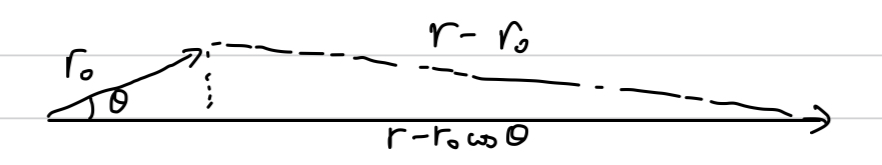
\includegraphics[width=0.5\linewidth]{src/vector difference approx.jpeg}
    \caption{Intuition for $|\mbf r - \mbf r'|\approx r - r'\cos\theta$}
    \label{fig:vector difference approx}
\end{figure}
This is an approximation up to the first order of $r'/r$. 
Let $\mbf k = k\hat r$, then 
\[ 
    e^{ik|\mbf r - \mbf r'|} \approx e^{ikr}e^{i\mbf{k\cdot r'}} 
    \implies \df{e^{ik|\mbf{r - r'}}|}{|\mbf{r-r'}|} \approx 
    \df{e^{ikr}}{r}e^{-i\mbf{k\cdot r'}} 
    % \approx \df{e^{ikr}}{r}\left(1 - i\mbf k\cdot \mbf r'\right)
\] 
Substituting into equation~\ref{eqn:integral se} with the free 
solution $\psi_0=e^{ikz}$ reads 
\leqalign{eqn:far born integral}{
    \psi(\mbf r) \approx e^{ikz} - 
    \df{m}{2\pi \hb^2} \df{e^{ikr}}{r}\int e^{-i\mbf{k\cdot r'}}
    V(\mbf r')\psi(\mbf r')\, d^3\mbf r'
}
Equation~\ref{eqn:far born integral} is ``exact'' to the first 
order in $r'/r$, so it is actually exact for the purposes of calculating the 
scattering amplitudes, which are at asymptotically large $r$. 
Equation~\ref{eqn:far born integral} 
standard form of the eigenstate in the radiation zone. 
Recall from~\ref{eqn:radiation state} that the scattering amplitudes 
are the coefficients of $Ae^{ikr}/r$ at large $r$, we 
can read off their \textit{exact} values 
\leqalign{eqn:wave amplitude equation}{
    f(\theta, \phi) = -\df{m}{2\pi \hb^2A}\int e^{-i\mbf{k\cdot r'}}V(\mbf r')\psi(\mbf r')d^3\mbf r'
}
Note that the right hand side contains $\psi$ so this is not a closed form. 
The Born approximation assumes that the incoming 
wave is not substantially altered by the scattering, 
so 
\[ 
    \psi(\mbf r')\approx \psi_0(\mbf r') = Ae^{ikz'} = Ae^{i\mbf k'\cdot \mbf r'}, \quad \mbf k' = k\hat z 
\] 
This yields the first Born approximation for scattering amplitudes. 
The following holds when \textit{the incident energy is large compared to the potential}. 
\begin{mdframed}\leqalign{eqn:first born approximation}{
    f(\theta, \phi) \approx -\df{m}{2\pi \hb^2} 
    \int e^{i\mbf{(k' - k)\cdot r'}}V(\mbf r')d^3\mbf r', \quad \mbf k' = k\hat z, \mbf k = k\hat r_{\theta, \phi}
}\end{mdframed}
Note that $\mbf k'$ points in the direction of the incident beam, 
while $\mbf k$ points in the scattering direction. 
Additionally, \textit{when the energy of the incident beam is low} 
so that the wavelength is large compared to the 
scattering region, $e^{i\mbf{(k-k')\cdot r'}}$ is essentially constant over $\mbf r'$ 
for which $V(\mbf r')$ is significant, in which case 
\leqalign{eqn:low energy born approx}{
    f(\theta, \phi) \approx -\df{m}{2\pi \hb^2}\int V(\mbf r')\, d^3\mbf r'
}
When the potential is spherically symmetric, the first 
Born approximation~\ref{eqn:first born approximation}
may be explicitly evaluated. The following equation does not require low incident energy, 
only the Born condition that the incident energy is large compared to the potential. 
\begin{mdframed}
    \leqalign{eqn:spherical low energy born approx}{
        f(\theta) \approx -\df{2m}{\hb^2\kappa} \int_0^\infty rV(r)\sin(\kappa r)\, dr, 
        \quad \kappa = 2k\sin(\theta/2)
    }    
\end{mdframed}